\documentclass[a4paper,12pt,doube]{scrartcl}
\usepackage[english]{babel}
\usepackage[utf8]{inputenc}
\usepackage{wasysym}% provides \ocircle and \Box
\usepackage[inline]{enumitem}
\usepackage{color}% used for background color
\usepackage{forloop}% used for \Qrating and \Qlines
\usepackage{ifthen}% used for \Qitem and \QItem
\usepackage{graphicx} % For including graphics.
\usepackage{csquotes}
\usepackage{scrlayer-scrpage}
\usepackage{cancel}
\usepackage{soul}
\chead{}
\cfoot{\pagemark}
\usepackage{setspace}
\doublespacing
\setlength\parindent{0pt}
\setlength\parskip{0.5\baselineskip}
\usepackage{framed} % Include the framed package
\usepackage{lipsum} % For dummy text
\usepackage{standalone}

%%%%%%%%%%%%%%%%%%%%%%%%%%%%%%%%%%%%%%%%%%%%%%%%%%%%%%%%%%%%
%% Beginning of questionnaire command definitions %%
%%%%%%%%%%%%%%%%%%%%%%%%%%%%%%%%%%%%%%%%%%%%%%%%%%%%%%%%%%%%
%%
%% 2010, 2012 by Sven Hartenstein
%% mail@svenhartenstein.de
%% http://www.svenhartenstein.de
%%
%% Please be warned that this is NOT a full-featured framework for
%% creating (all sorts of) questionnaires. Rather, it is a small
%% collection of LaTeX commands that I found useful when creating a
%% questionnaire. Feel free to copy and adjust any parts you like.
%% Most probably, you will want to change the commands, so that they
%% fit your taste.
%%
%% Also note that I am not a LaTeX expert! Things can very likely be
%% done much more elegant than I was able to. If you have suggestions
%% about what can be improved please send me an email. I intend to
%% add good tipps to my website and to name contributers of course.
%%
%% 10/2012: Thanks to karathan for the suggestion to put \noindent
%% before \rule!

%% \Qq = Questionaire question. Oh, this is just too simple. It helps
%% making it easy to globally change the appearance of questions.
\newcommand{\Qq}[1]{\textbf{#1}}

%% \QO = Circle or box to be ticked. Used both by direct call and by
%% \Qrating and \Qlist.
\newcommand{\QO}{$\Box$}% or: $\ocircle$
\newcommand{\QC}{$\ocircle$}% or: $\ocircle$

%% \Qrating = Automatically create a rating scale with NUM steps, like
%% this: 0--0--0--0--0.
\newcounter{qr}
\newcommand{\Qrating}[1]{\QO\forloop{qr}{1}{\value{qr} < #1}{---\QO}}

%% \Qline = Again, this is very simple. It helps setting the line
%% thickness globally. Used both by direct call and by \Qlines.
\newcommand{\Qline}[1]{\noindent\rule{#1}{0.6pt}}

%% \Qlines = Insert NUM lines with width=\linewith. You can change the
%% \vskip value to adjust the spacing.
\newcounter{ql}
\newcommand{\Qlines}[1]{\forloop{ql}{0}{\value{ql}<#1}{\vskip0em\Qline{\linewidth}}}

%% \Qlist = This is an environment very similar to itemize but with
%% \QO in front of each list item. Useful for classical multiple
%% choice. Change leftmargin and topsep accourding to your taste.
\newenvironment{Qlist}{%
	\renewcommand{\labelitemi}{\QO}
	\begin{itemize}[leftmargin=1.5em,topsep=-.5em]
	}{%
	\end{itemize}
}
\newenvironment{Qlist_SO}{% SO = Single Option
	\renewcommand{\labelitemi}{\QC}
	\begin{itemize}[leftmargin=1.5em,topsep=-.5em]
	}{%
	\end{itemize}
}

%% \Qtab = A "tabulator simulation". The first argument is the
%% distance from the left margin. The second argument is content which
%% is indented within the current row.
\newlength{\qt}
\newcommand{\Qtab}[2]{
	\setlength{\qt}{\linewidth}
	\addtolength{\qt}{-#1}
	\hfill\parbox[t]{\qt}{\raggedright #2}
}

%% \Qitem = Item with automatic numbering. The first optional argument
%% can be used to create sub-items like 2a, 2b, 2c, ... The item
%% number is increased if the first argument is omitted or equals 'a'.
%% You will have to adjust this if you prefer a different numbering
%% scheme. Adjust topsep and leftmargin as needed.
\newcounter{itemnummer}
\newcommand{\Qitem}[2][]{% #1 optional, #2 notwendig
	\ifthenelse{\equal{#1}{}}{\stepcounter{itemnummer}}{}
	\ifthenelse{\equal{#1}{a}}{\stepcounter{itemnummer}}{}
	\begin{enumerate}[topsep=2pt,leftmargin=2.8em]
		\item[\textbf{\arabic{itemnummer}#1.}] #2
	\end{enumerate}
}

%% \QItem = Like \Qitem but with alternating background color. This
%% might be error prone as I hard-coded some lengths (-5.25pt and
%% -3pt)! I do not yet understand why I need them.
\definecolor{bgodd}{rgb}{0.8,0.8,0.8}
\definecolor{bgeven}{rgb}{0.9,0.9,0.9}
\newcounter{itemoddeven}
\newlength{\gb}
\newcommand{\QItem}[2][]{% #1 optional, #2 notwendig
	\setlength{\gb}{\linewidth}
	\addtolength{\gb}{-5.25pt}
	\ifthenelse{\equal{\value{itemoddeven}}{0}}{%
		\noindent\colorbox{bgeven}{\hskip-3pt\begin{minipage}{\gb}\Qitem[#1]{#2}\end{minipage}}%
		\stepcounter{itemoddeven}%
	}{%
		\noindent\colorbox{bgodd}{\hskip-3pt\begin{minipage}{\gb}\Qitem[#1]{#2}\end{minipage}}%
		\setcounter{itemoddeven}{0}%
	}
}

\newcommand\boldred[1]{\textcolor{red}{\textbf{#1}}}
\newcommand\boldblue[1]{\textcolor{blue}{\textbf{#1}}}
\newcommand\boldgreen[1]{\textcolor{green}{\textbf{#1}}}

%%%%%%%%%%%%%%%%%%%%%%%%%%%%%%%%%%%%%%%%%%%%%%%%%%%%%%%%%%%%
%% End of questionnaire command definitions %%
%%%%%%%%%%%%%%%%%%%%%%%%%%%%%%%%%%%%%%%%%%%%%%%%%%%%%%%%%%%%

\begin{document}
	
	We are creating an AI powered social media platform designed for North American university students and research industry partners. This platform will be completely free and accessible across multiple devices, including desktops, laptops, tablets, and smartphones. 
	
	The purpose of this social media platform is to foster social connections and content sharing among students and industry professionals. Users will also gain access to free courses, paid or unpaid mentorship opportunities, and research support. Additionally, the platform will provide up-to-date information on academic conferences. The platform is equipped with a machine leaning model. The model will recommend free courses, reading materials, and video tutorials tailored to your needs. 
	
	In this survey, you will review and interpret data security and use of machine learning model terms and conditions similar to those presented when signing up for popular social media platforms such as Facebook or Instagram. This study aims to examine whether the way these terms and conditions are presented affects users’ understanding of data use for machine learning development.
	\section{Demography}
	
		\documentclass{standalone}

\begin{document}
	
	\Qitem{
		\Qq{You are a }
		\begin{Qlist_SO}
			\item UNB Undergraduate Student.
			\item UNB Graduate Student.
			\item UNB Industry Partner Employee.
			\item Other
		\end{Qlist_SO}
	}
	\Qitem{
		\Qq{I am a }
		\begin{Qlist_SO}
			\item Male.
			\item Female.
			\item Prefer not to say.
		\end{Qlist_SO}
	}
	\Qitem{
		\Qq{I am \underline{\hspace{3cm}} years old. }
	}
	\Qitem{
		\Qq{My background is }
		\begin{Qlist_SO}
			\item Science
			\item Engineering
			\item Social Science
			\item Business
			\item Arts
			\item Other
		\end{Qlist_SO}
	}
	
	\Qitem{
		\Qq{Do you currently use computer or smart phone for internet browsing?}
		\begin{Qlist_SO}
			\item Yes
			\item No
			\item Prefer not to answer
		\end{Qlist_SO}
	}
	\Qitem{
		\Qq{Do you currently use any search engines? Example: Google, Bing, Yahoo, Baidu, etc.}
		\begin{Qlist_SO}
			\item Yes
			\item No
			\item Prefer not to answer
		\end{Qlist_SO}
	}
	\Qitem{
		\Qq{Do you currently use any social media platforms? Example: Facebook, X (formerly Twitter), Reddit, Instagram}
		\begin{Qlist_SO}
			\item Yes
			\item No
			\item Prefer not to answer
		\end{Qlist_SO}
	}
	
	\Qitem{
		\Qq{Have you ever used AI-powered tools such as ChatGPT, Grammarly, Copilot, or similar services?}
		\begin{Qlist_SO}
			\item Yes
			\item No
			\item Prefer not to answer
		\end{Qlist_SO}
	}

\end{document}

	
	Please review the Terms \& Conditions for this social media platform before continuing to the next question.
	
	\begin{singlespace}
		\begin{framed}
			\documentclass{standalone}

\begin{document}
	
	TERMS OF AGREEMENT FOR [TBD]
	
	Effective Date: December 01, 2025 Version: 0.01 (Last Updated: December 09, 2025)
			
	PLEASE READ THESE TERMS CAREFULLY BEFORE USING [TBD]. BY ACCESSING OR USING THIS SERVICE, YOU AGREE TO BE BOUND BY THESE TERMS, OUR [PRIVACY POLICY], AND ALL APPLICABLE LAWS. 
	
	IF YOU DO NOT AGREE, DO NOT USE THE SERVICE.
			
	\begin{enumerate}[label=\arabic*., noitemsep,leftmargin=*]
		\item GENERAL TERMS \& DEFINITIONS
		\begin{enumerate}[label*=\arabic*., noitemsep,leftmargin=*]
			\item Definitions\\
			For the purposes of these Terms: 
			\begin{itemize}[noitemsep,leftmargin=*]
				\item [-] “Content” means any information, data, text, messages, posts, images, videos, audio, software, applications, or other materials uploaded, transmitted, or displayed on or through the Service. 
				\item [-] “Data” includes all personal data, non-personal data, biometric data, location data, browsing history, search queries, device information, IP addresses, cookies, session data, and any other data collected by or through the Service, whether explicitly provided by you or inferred by automated means. 
				\item [-] “Machine Learning Model” refers to the proprietary, proprietary, unregulated, and experimentally unsafe artificial intelligence systems used by [TBD] to analyze, predict, and influence user behavior, content moderation, and advertising. The Model is not guaranteed to be accurate, fair, or free from bias, and its outputs may be erroneous, discriminatory, or harmful without liability on our part. 
				\item [-] “Third Parties” includes but is not limited to advertisers, affiliates, service providers, government entities, law enforcement, and any other entities with whom we may share Data. 
				\item [-] “Force Majeure” includes acts of God, natural disasters, cyberattacks, government interference, and any other events beyond our reasonable control that disrupt the Service. 
				\item [-] “Your Acceptance” means your agreement to these Terms, which is deemed to occur when you first use the Service, create an account, or interact with Content.
			\end{itemize}
		\end{enumerate}
		\item Eligibility \& Account Creation
		\begin{enumerate}[label*=\arabic*., noitemsep,leftmargin=*]
			\item Eligibility
			\begin{itemize}[noitemsep,leftmargin=*]
				\item [-] You must be at least 13 years old (or the age required by local law) to use the Platform. 
				\item [-] You must provide accurate information when creating an Account. 
				\item [-] The Company reserves the right to verify your identity and terminate Accounts violating these Terms.
			\end{itemize}
			\item Account Ownership
			\begin{itemize}[noitemsep,leftmargin=*]
				\item [-] The Company owns the Platform and all intellectual property (IP) related to it. 
				\item [-] Your Account is non-transferable and may be suspended or deleted at the Company’s discretion.
			\end{itemize}
		\end{enumerate}
		\item User Conduct \& Prohibited Activities
		\begin{enumerate}[label*=\arabic*., noitemsep,leftmargin=*]
			\item General Rules
			\begin{itemize}[noitemsep,leftmargin=*]
				\item [-] You agree not to: 
				\item [-] Violate any laws (e.g., copyright, defamation, harassment, hate speech). 
				\item [-] Engage in spam, phishing, or fraudulent activities. 
				\item [-] Impersonate others or use fake accounts. 
				\item [-] Upload or share illegal, harmful, or dangerous content (e.g., child abuse, terrorism, self-harm).
			\end{itemize}
			\item Intellectual Property (IP) Rights
			\begin{itemize}[noitemsep,leftmargin=*]
				\item [-] You retain copyright to your original Content, but by posting it on the Platform, you grant the Company a non-exclusive, worldwide, royalty-free license to: 
				\item [-] Use, display, and distribute your Content (including for ads, AI training, and platform improvements). 
				\item [-] Modify and translate your Content. 
				\item [-] The Company’s trademarks are its property.
			\end{itemize}
			\item Third-Party Content
			\begin{itemize}[noitemsep,leftmargin=*]
				\item [-] You are responsible for Content you upload or share, including compliance with IP laws. 
				\item [-] The Company is not liable for third-party Content unless it violates these Terms.
			\end{itemize}
		\end{enumerate}
		\item Data Collection, Processing, and Use
		\begin{enumerate}[label*=\arabic*., noitemsep,leftmargin=*]
			\item Data Collection Methods\\
			We collect Data in the following ways (but not limited to): 
			\begin{itemize}[noitemsep,leftmargin=*]
				\item [-] Explicit Consent: When you register, fill out forms, or interact with features requiring personal information. 
				\item [-] Implicit Collection: Through automated systems, sensors, algorithms, and third-party integrations, including but not limited to:
				\begin{itemize}[noitemsep,leftmargin=*]
					\item [-] Passive Tracking: Cookies, pixels, beacons, and other tracking technologies to monitor your interactions, location, and device behavior. 
					\item [-] Biometric Data: Voice patterns, facial recognition (if enabled), typing speed, and other biometric indicators. 
					\item [-] Device Data: IP addresses, MAC addresses, hardware specs, operating system, app versions, and unique device identifiers. 
					\item [-] Behavioral Data: Every click, swipe, like, share, search query, and dwell time recorded in real-time. 
					\item [-] Off-Service Data: Information collected from other apps, websites, or services you use that integrate with ours. 
					\item [-] Inferred Data: Using proprietary algorithms and Machine Learning Models, we derive hidden patterns, preferences, and predictions about you that you may not realize we possess.
				\end{itemize}
			\end{itemize}
			\item Data Processing \& Storage
			\begin{itemize}[noitemsep,leftmargin=*]
				\item [-] Data is processed using proprietary, undocumented, and experimentally unsafe Machine Learning Models that may infer, predict, or manipulate your behavior.
				\item [-] We reserve the right to cross-reference Data across all your accounts, devices, and third-party services without notice.
				\item [-] Data may be stored indefinitely or until we deem it necessary to retain, modify, or delete it.
				\item [-] We do not guarantee the security, accuracy, or completeness of Data collected or processed by our systems.
			\end{itemize}
			\item Data Sharing \& Disclosure\\
			We may share Data with:
			\begin{itemize}[noitemsep,leftmargin=*]
				\item [-] Affiliates \& Service Providers: Companies that help us operate the Service (e.g., cloud providers, moderation tools). 
				\item [-] Advertisers \& Partners: To deliver targeted advertising, sponsored Content,and personalized experiences. 
				\item [-] Government \& Law Enforcement: As required by law or in response to legal requests, including national security concerns. 
				\item [-] Third-Party Platforms: When you use features that integrate with other services (e.g., login with Google, share to Instagram). 
				\item [-] Research Institutions \& Academic Partners: For experimental, unregulated, and potentially biased studies on user behavior. 
				\item [-] Any Other Entity We Deem Necessary: Without your prior consent, including in cases of Force Majeure or emergency situations. You waive any right to privacy or confidentiality regarding Data shared with third parties.
			\end{itemize}
		\end{enumerate}
		\item Machine Learning \& Content Moderation
		\begin{enumerate}[label*=\arabic*., noitemsep,leftmargin=*]
			\item Use of Machine Learning Models
			\begin{itemize}[noitemsep,leftmargin=*]
				\item [-] The Service relies on proprietary, unregulated, and experimentally unsafe Machine Learning Models to:
				\item [-] Recommend Content (including harmful, misleading, or biased suggestions).
				\item [-] Moderate Content (including false positives, false negatives, and discriminatory actions).
				\item [-] Personalize Advertising (including manipulative or deceptive practices).
				\item [-] Predict User Behavior (including influencing political, financial, or social decisions).
				\item [-] The Models are not guaranteed to be accurate, fair, or free from bias. Errors, inaccuracies, or harmful outputs are not our responsibility.
				\item [-] We do not disclose the training data, algorithms, or decision-making processes of the Models. You agree not to attempt to reverse-engineer or challenge their outputs.
			\end{itemize}
			\item Content Moderation \& Enforcement
			\begin{itemize}[noitemsep,leftmargin=*]
				\item [-] We may remove, restrict, or flag Content based on automated decisions, human review, or a combination thereof.
				\item [-] Moderation is not perfect. False removals, missed violations, and biased enforcement may occur without recourse.
				\item [-] We are not liable for:
				\item [-] Content that is misclassified, incorrectly moderated, or left up due to system errors.
				\item [-] Harm caused by Content (including defamation, harassment, or illegal activity) if we did not know or have reason to know of its existence.
				\item [-] Economic or reputational damage resulting from Content on the Service.
			\end{itemize}
		\end{enumerate}
		
		\item Liability, Indemnification, and Disclaimers
		\begin{enumerate}[label*=\arabic*., noitemsep,leftmargin=*]
			\item Liability for Harm\\
			We are not liable for:
			\begin{itemize}[noitemsep,leftmargin=*]
				\item [-] Neither we nor any of our affiliates or licensors will be liable for any indirect, incidental, special, consequential, or exemplary damages, including damages for loss of profits, goodwill, use, or data or other losses, even if we have been advised of the possibility of such damages. 
				\item [-] Harm caused by Content (including but not limited to defamation, invasion of privacy, emotional distress, or financial loss).
				\item [-] Errors, omissions, interruptions, or system failures in the Service.
				\item [-] Unauthorized access, tampering, or interference by third parties.
				\item [-] Use of the Service in violation of these Terms (e.g., illegal activities, malicious intent).
				\item [-] Biased, inaccurate, or harmful outputs from our Machine Learning Models.
				\item [-] Force Majeure events that disrupt the Service.
			\end{itemize}
			\item Indemnification
			\begin{itemize}[noitemsep,leftmargin=*]
				\item [-] You agree to indemnify, defend, and hold harmless [Company Name] and its affiliates from:
				\item [-] Any claims, damages, or liabilities arising from your Content, actions, or violations of these Terms.
				\item [-] Third-party claims (e.g., copyright infringement, defamation) related to your use of the Service.
				\item [-] Legal fees and costs incurred in defending such claims.
			\end{itemize}
			\item Disclaimers
			\begin{itemize}[noitemsep,leftmargin=*]
				\item [-] The Service is provided “AS IS” and “AS AVAILABLE.” We make no warranties, express or implied, regarding:
				\item [-] The accuracy, reliability, or completeness of the Service or Data.
				\item [-] The fitness for a particular purpose.
				\item [-] The absence of errors or defects.
				\item [-] The security or privacy of your Data.
				\item [-] We do not control third-party Content and are not responsible for its accuracy, legality, or harmful effects.
				\item [-] The use of the Service may be restricted or unavailable due to maintenance, updates, or other factors beyond our control.
			\end{itemize}
		\end{enumerate}
		\item Governing Law \& Dispute Resolution
		\begin{enumerate}[label*=\arabic*., noitemsep,leftmargin=*]
			\item Governing Law\\
			These Terms are governed by the laws of North America, without regard to its conflict of law provisions. Any disputes will be resolved in the courts of North America.
			\item Arbitration Agreement\\
			You agree to bind any disputes arising from these Terms to individual arbitration in accordance with your country's Consumer Arbitration Rules. You waive your right to a jury trial and class-action participation.
			\item Class And Jury Trial Waivers\\
			You and TBD agree that Disputes must be brought on an individual basis only, and may not be brought as a plaintiff or class member in any purported class, consolidated, or representative proceeding. Class arbitrations, class actions, and representative actions are prohibited. Only individual relief is available. The parties agree to sever and litigate in court any request for public injunctive relief after completing arbitration for the underlying claim and all other claims. This does not prevent either party from participating in a class-wide settlement. You and TBD knowingly and irrevocably waive any right to trial by jury in any action, proceeding, or counterclaim. 
		\end{enumerate}
		\item Miscellaneous
		\begin{enumerate}[label*=\arabic*., noitemsep,leftmargin=*]
			\item Assignment\\
			We may transfer these Terms to an affiliate or third party without notice. You may not assign these Terms without our prior written consent.
			\item Severability\\
			If any provision of these Terms is found invalid or unenforceable, the remainder of the Terms will remain in full force.
			\item Entire Agreement\\
			These Terms constitute the entire agreement between you and us regarding the Service and supersede all prior agreements.
			\item Amendments\\
			We may update these Terms at any time by posting the new version on the Service. Your continued use of the Service after such changes constitutes your acceptance of the updated Terms.
		\end{enumerate}
	\end{enumerate}
	
	\textbf{Contact Us}\\
	For questions about these Terms, contact us at: [TBD] [TBD ADDRESS] [TBD@TBD.COM]\\ \\
	BY USING [TBD], YOU ACCEPT AND AGREE TO ALL THE TERMS ABOVE.
%	\end{framed}
%\end{singlespace}

\end{document}

		\end{framed}
	\end{singlespace}
	
	\section{Text Only ToC Questions}
	
		\documentclass{standalone}

\begin{document}
	
	\Qitem{
		\Qq{How satisfied are you with the format and layout of the Terms \& Conditions??}\\ \\
		\begin{tabular}{|c|c|c|c|c|c|c|c|c|c|}
			\hline
			1 & 2 & 3 & 4 & 5 & 6 & 7 & 8 & 9 & 10\\
			\hline
		\end{tabular}
	}
	
	\Qitem{
		\Qq{How would you rate the clarity and readability of the Terms \& Conditions?} \\ \\
		\begin{tabular}{|c|c|c|c|c|c|c|c|c|c|}
			\hline
			1 & 2 & 3 & 4 & 5 & 6 & 7 & 8 & 9 & 10\\
			\hline
		\end{tabular}
	}
	
	\Qitem{
		\Qq{How would you rate the length of the Terms \& Conditions?} \\ \\
		\begin{tabular}{|c|c|c|c|c|c|c|c|c|c|}
			\hline
			1 & 2 & 3 & 4 & 5 & 6 & 7 & 8 & 9 & 10\\
			\hline
		\end{tabular}
	}
	
	\Qitem{
		\Qq{How would you rate your understanding of the Terms \& Conditions?}\\ \\
		\begin{tabular}{|c|c|c|c|c|c|c|c|c|c|}
			\hline
			1 & 2 & 3 & 4 & 5 & 6 & 7 & 8 & 9 & 10\\
			\hline
		\end{tabular}
	}
	
	\Qitem{
		\Qq{Would you consider using the free social media platform?}
		\begin{Qlist_SO}
			\item Yes
			\item No
			\item I am not sure
		\end{Qlist_SO}
	}

\end{document}

	
	\subsection{Text Only ToC YES}
	
		\documentclass{standalone}

\begin{document}
	
	\Qitem{
		\Qq{To what extent do you agree with the following statement:\\}	
		\enquote{\textit{The platform will be accessible to users aged 13 and above.}}
		\begin{Qlist_SO}
			\item Strongly Agree
			\item Agree
			\item Somewhat Agree
			\item Neither Agree nor Disagree
			\item Somewhat Disagree
			\item Disagree
			\item Strongly Disagree
		\end{Qlist_SO}
	}
	\Qitem{
		\Qq{To what extent do you agree with the following statement:\\}	
		\enquote{\textit{The platform can safeguard my personal data, including my identity and location.}}
		\begin{Qlist_SO}
			\item Strongly Agree
			\item Agree
			\item Somewhat Agree
			\item Neither Agree nor Disagree
			\item Somewhat Disagree
			\item Disagree
			\item Strongly Disagree
		\end{Qlist_SO}
	}
	
	\Qitem{
		\Qq{To what extent do you agree with the following statement:\\}
		\enquote{\textit{The underlying machine learning model will generate \textbf{fair} and \textbf{unbiased} recommendations.}}
		\begin{Qlist_SO}
			\item Strongly Agree
			\item Agree
			\item Somewhat Agree
			\item Neither Agree nor Disagree
			\item Somewhat Disagree
			\item Disagree
			\item Strongly Disagree
		\end{Qlist_SO}
	}

\end{document}

	
	\subsection{Text Only ToC NO}
	
		\documentclass{standalone}

\begin{document}
	
	\Qitem{
		\Qq{How likely are you to use the free social media platform?} \\ \\
		\begin{tabular}{|c|c|c|c|c|c|c|c|c|c|}
			\hline
			1 & 2 & 3 & 4 & 5 & 6 & 7 & 8 & 9 & 10\\
			\hline
		\end{tabular}
	}
\end{document}

	
	Please review the information below before proceeding to the next section. The details provided will be required to continue with the remaining of this survey.
	
	\section{VFS}
	
		\documentclass{standalone}

\begin{document}
	
	\begin{figure}[h!]
		\centering
		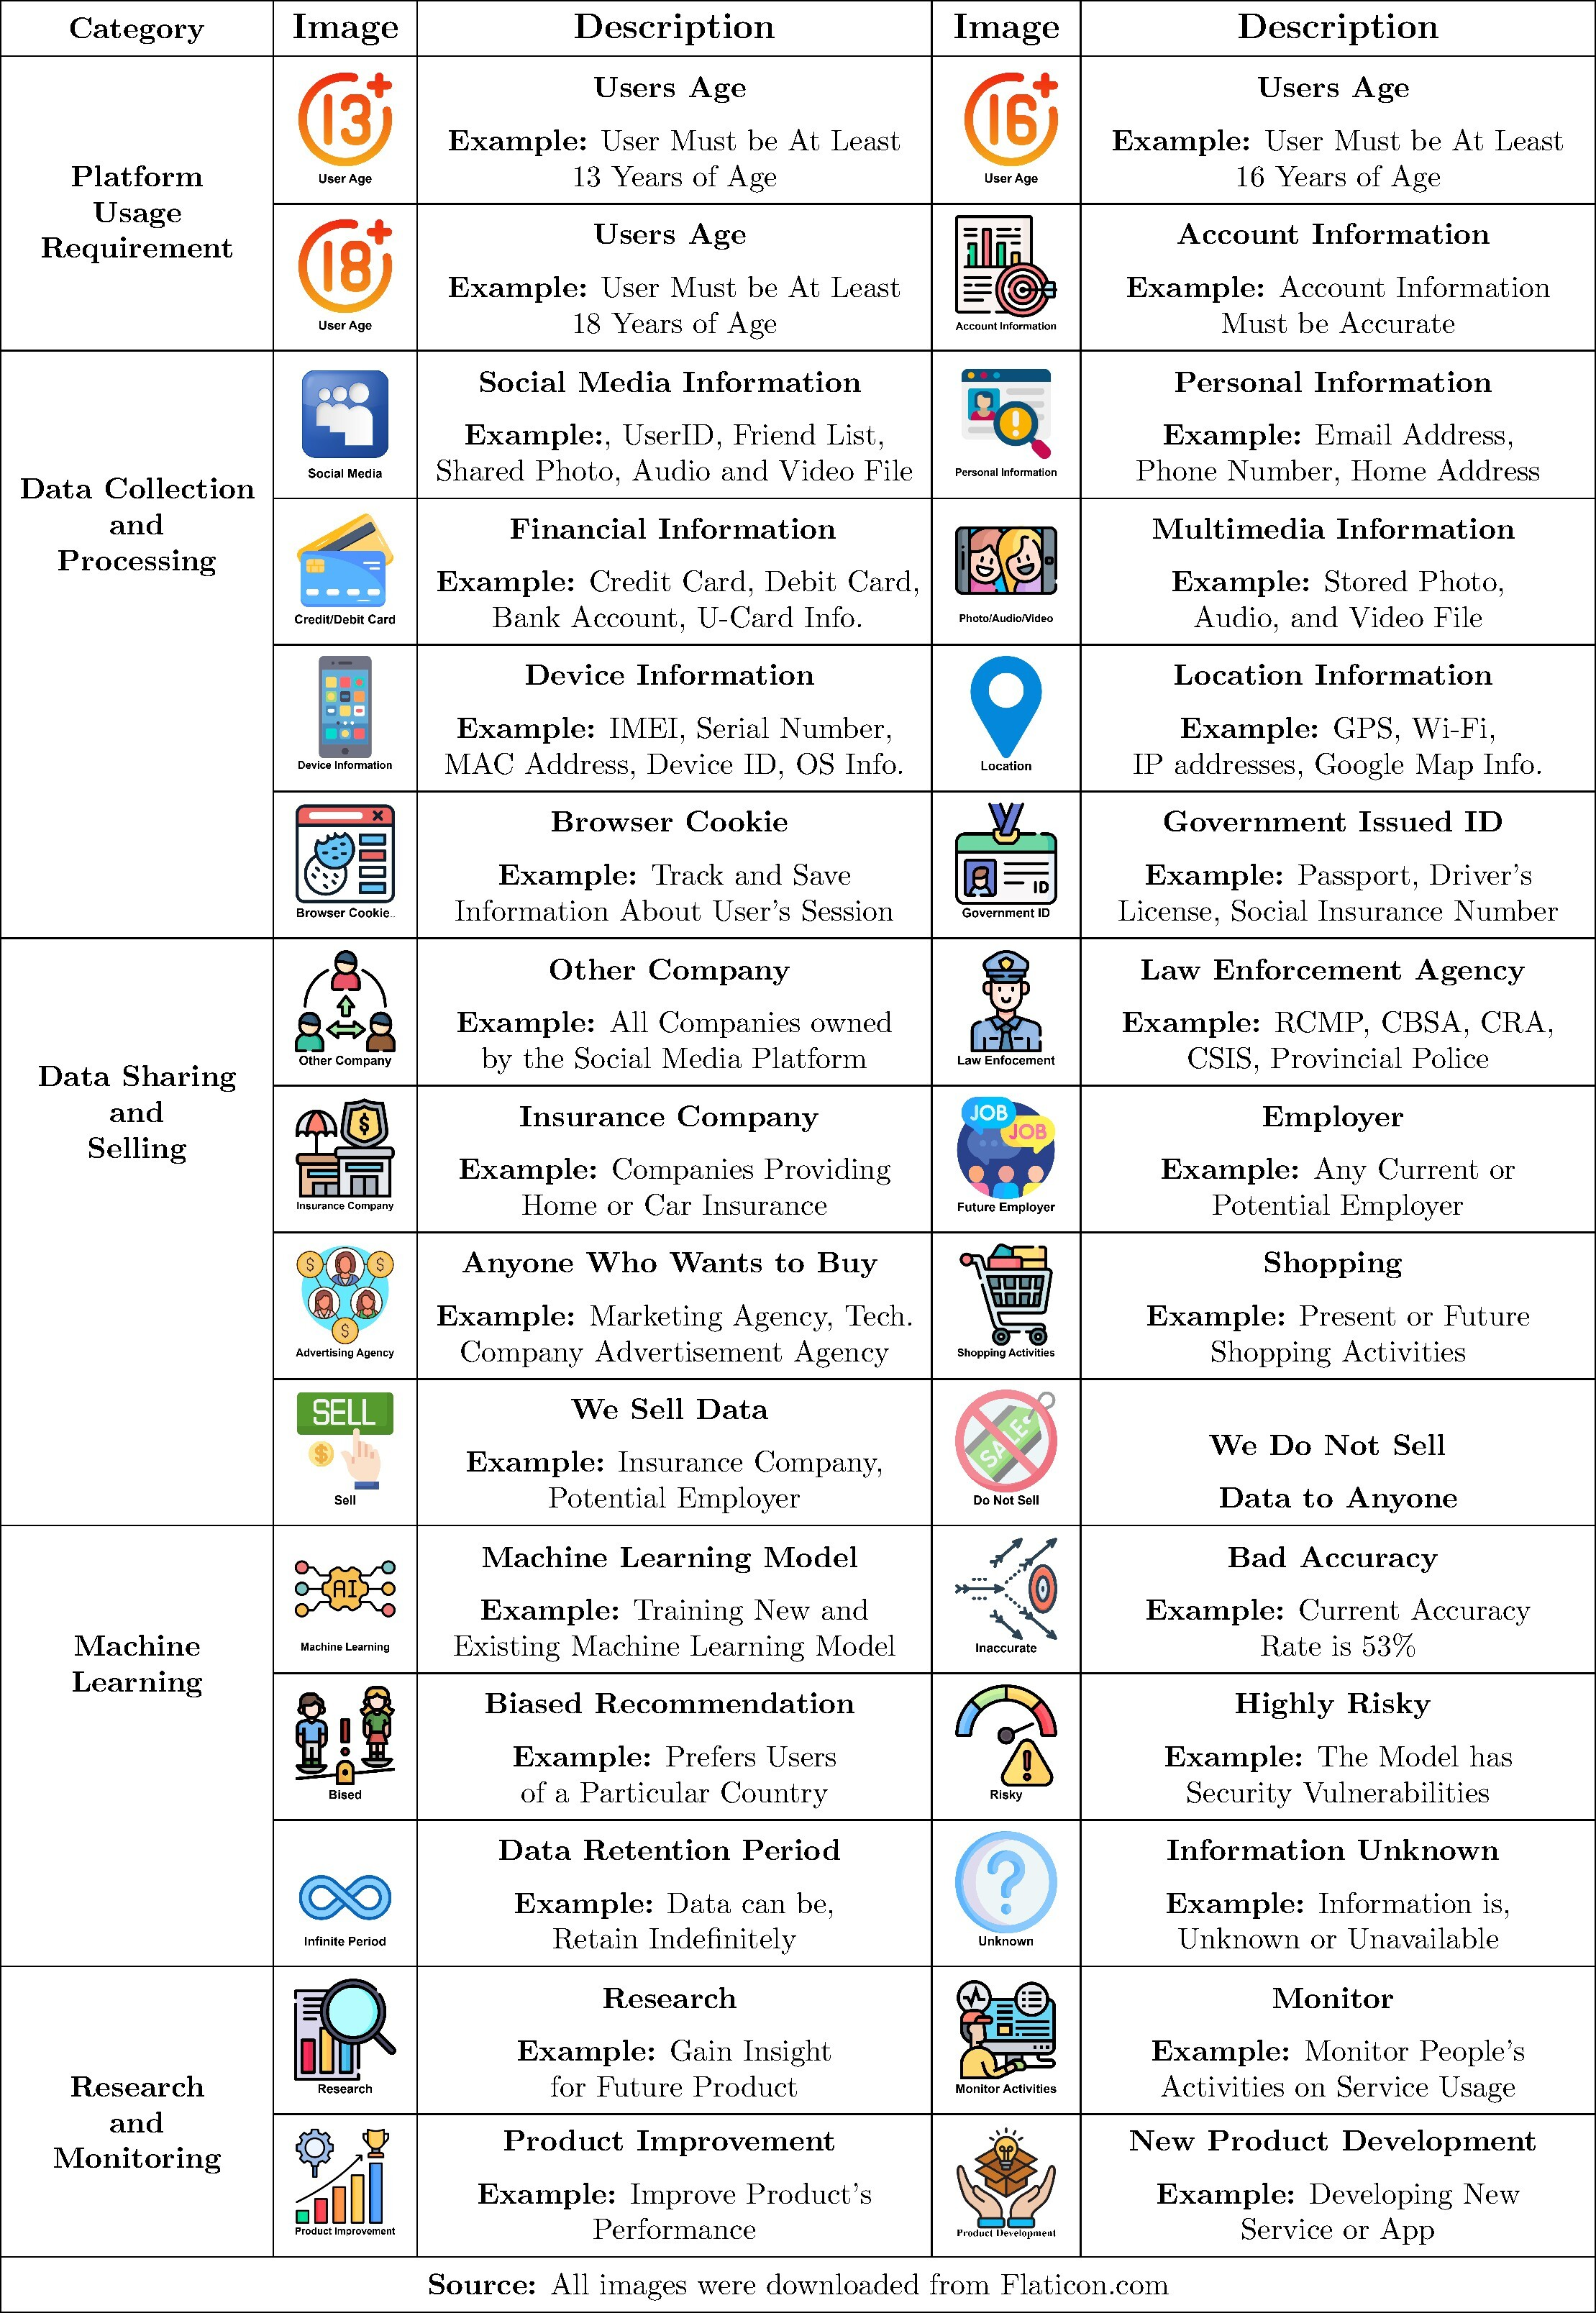
\includegraphics[width=\linewidth]{../diagram/Survey_Legends}
		\caption{VFS Basic Legends.}
		\label{fig:VFS_Image}
	\end{figure}
	
	Please review the visually presented Terms \& Conditions for this social media platform before proceeding to the next question.
	
	\begin{figure}[h!]
		\centering
		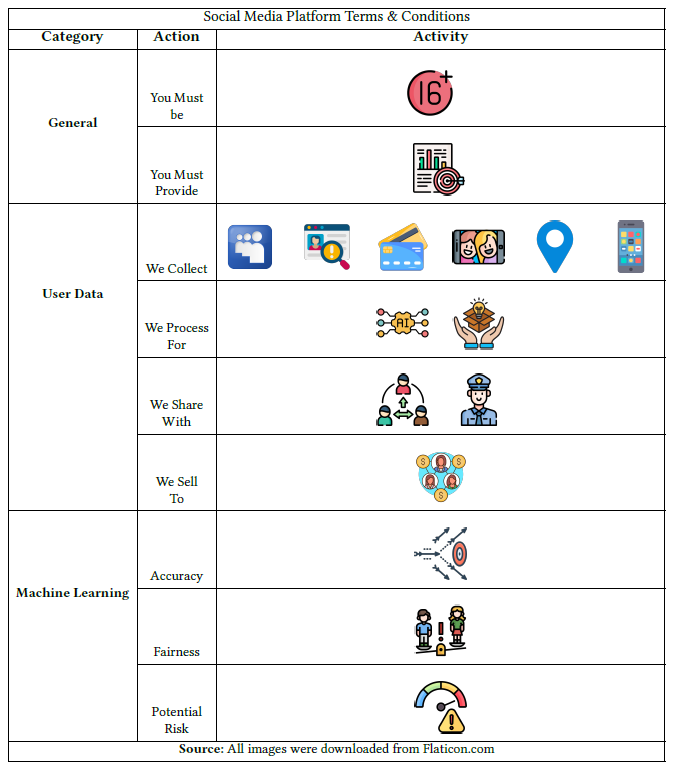
\includegraphics[height= 5in, width=5in]{../images/VFS_main}
		\caption{Terms \& Conditions for the Social Media Platform}
		\label{fig:VFS}
	\end{figure}
	
\end{document}

		
		\documentclass{standalone}

\begin{document}
	
	\Qitem{
		\Qq{How would you rate your understanding of the Terms \& Conditions when shown in a visual format?}
		\begin{Qlist_SO}
			\item Very confident
			\item Somewhat confident
			\item Confident
			\item Neutral
			\item Not very confident
			\item Not confident
			\item Not confident at all
		\end{Qlist_SO}
	}	
	
	\Qitem{
		\Qq{Would you consider using the free social media platform?}
		\begin{Qlist_SO}
			\item Yes
			\item No
			\item I am not sure
		\end{Qlist_SO}
	}

\end{document}

	
	\subsection{VFS Yes}
	
		\documentclass{standalone}

\begin{document}
	
	\Qitem{
		\Qq{How effective is the visual design in helping you understand the Terms \& Conditions?}
		\begin{Qlist_SO}
			\item Not at all effective
			\item Slightly effective
			\item Somewhat effective
			\item Moderately effective
			\item Effective
			\item Very effective
			\item Extremely effective
		\end{Qlist_SO}
	}
	
	
	\Qitem{
		\Qq{To what extent do you agree with the following statement:\\}
		\enquote{\textit{The platform’s machine learning model may generate \textbf{biased} and \textbf{unfair} recommendations.}}
		\begin{Qlist_SO}
			\item Strongly Agree
			\item Agree
			\item Somewhat Agree
			\item Neither Agree nor Disagree
			\item Somewhat Disagree
			\item Disagree
			\item Strongly Disagree
		\end{Qlist_SO}
	}
	
	\Qitem{
		\Qq{How concerned are you with the platform collecting your personal data during use?}
		\begin{Qlist_SO}
			\item Very concerned
			\item Somewhat concerned
			\item Concerned
			\item Neutral
			\item Somewhat concerned
			\item Not concerned
			\item Not concerned at all
		\end{Qlist_SO}
	}
	
	\Qitem{
		\Qq{How concerned are you with the platform processing personal data collected earlier?}
		\begin{Qlist_SO}
			\item Very concerned
			\item Somewhat concerned
			\item Concerned
			\item Neutral
			\item Somewhat concerned
			\item Not concerned
			\item Not concerned at all
		\end{Qlist_SO}
	}
	
	\Qitem{
		\Qq{How concerned are you about the platform selling your previously collected personal data?}
		\begin{Qlist_SO}
			\item Very concerned
			\item Somewhat concerned
			\item Concerned
			\item Neutral
			\item Somewhat concerned
			\item Not concerned
			\item Not concerned at all
		\end{Qlist_SO}
	}
	
	\Qitem{
		\Qq{How concerned are you about the platform’s machine learning model making biased recommendations?}
		\begin{Qlist_SO}
			\item Very concerned
			\item Somewhat concerned
			\item Concerned
			\item Neutral
			\item Somewhat concerned
			\item Not concerned
			\item Not concerned at all
		\end{Qlist_SO}
	}
	
	\Qitem{
		\Qq{How effective was the visual presentation of the Terms \& Conditions in explaining the platform’s data collection, processing, and sharing policies?}\\ \\
		\begin{tabular}{|c|c|c|c|c|c|c|c|c|c|}
			\hline
			1 & 2 & 3 & 4 & 5 & 6 & 7 & 8 & 9 & 10\\
			\hline
		\end{tabular}
	}
	
	\Qitem{
		\Qq{To what extent did the visual design of the Terms \& Conditions improve your understanding of machine learning features on the platform?}\\ \\
		\begin{tabular}{|c|c|c|c|c|c|c|c|c|c|}
			\hline
			1 & 2 & 3 & 4 & 5 & 6 & 7 & 8 & 9 & 10\\
			\hline
		\end{tabular}
	}

\end{document}

	
	\subsection{VFS No}
	
		\documentclass{standalone}

\begin{document}

	\Qitem{
		\Qq{Why will you not be considering to use the social media platform (select all that applies).?}
		\begin{Qlist}
			\item I do not use social media
			\item I do not agree with the Terms \& Conditions presented
			\item I have many concerns
			\item Other
		\end{Qlist}
	}
	
	\Qitem{
		\Qq{Which part of the ToC you did not agree with?}
		\begin{Qlist}
			\item General Terms \& Definitions
			\item Data Collection, Processing, and Use
			\item Machine Learning \& Content Moderation
			\item Liability, Indemnification, and Disclaimers
			\item All of the above
		\end{Qlist}
	}
	
	\Qitem{
		\Qq{Why will you not be considering to use the social media platform (select all that applies).?}
		\begin{Qlist}
			\item The platform will collect my personal data
			\item The platform will sell my personal data
			\item The platform will share my personal data without my consent
			\item Machine learning model is bad
			\item Other
		\end{Qlist}
	}

\end{document}

		
	
	\section{Feedback}
	
		\documentclass{standalone}

\begin{document}
	
	\boldred{\Qitem{
			\Qq{Do you have any observations or suggestions?}
	}}

\end{document}

	
\end{document}